
%BeginMC
\question

\begin{choices}
\correctchoice   %EndChoice
\choice  %EndChoice
\choice  %EndChoice
\choice  %EndChoice
\choice  %EndChoice
\end{choices}
%EndMC

%%%%%%%%%%%% Questions begin here. Copy and paste from template above.

%BeginMC
\question
Carefully compare relationships among these four trees. Which of the trees shows a different pattern of relationships than the other trees?

\begin{multicols}{2}

\begin{choices}
\choice Tree A. %dontshuffle%EndChoice
\choice Tree B. %dontshuffle%EndChoice
\correctchoice Tree C. %dontshuffle%EndChoice
\choice Tree D. %dontshuffle%EndChoice
\choice All four trees are identical. %dontshuffle%EndChoice
\end{choices}

\columnbreak

\begin{center}
\includegraphics[width=\columnwidth]{exam2_diff_trees}
\end{center}
\end{multicols}
%EndMC



%BeginMC
\question
Based upon the floral manipulation studies of columbine flowers, spurs act to maintain separate \textit{Aquilegia} species by\dots}

\begin{choices}
\correctchoice influencing pollen removal from and depositing on flowers. %EndChoice
\choice causing flowers to grow in different habitats. %EndChoice
\choice offering different rewards to different pollinators. %EndChoice
\choice attracting different pollinators. %EndChoice
\choice  %EndChoice
\end{choices}
%EndMC




%BeginMC
\begin{multicols}{2}
\question
The figure at right shows the average number of pollen grains remaining on \textit{Aquilegia pubescens} after visits by hawkmoths. Control flowers had normal length spurs. Shortened flowers had spurs that were cut short and tied by the researchers. Based on the figure, tell which, if any, type of reproductive isolation is supported by the data. 

\begin{choices}
	\correctchoice Mechanical isolation. %EndChoice
	\choice Temporal isolation. %EndChoice
	\choice Gametic isolation. %EndChoice
	\choice Habitat Isolation. %EndChoice
	\choice The figure does not provide support for the above types of reproductive isolation. %dontshuffle%EndChoice
\end{choices}

\columnbreak

	\includegraphics[width=0.45\textwidth]{/Users/goby/pictures/teach/163/case_studies/pollen_grains_remaining}
\end{multicols}
%EndMC

%BeginMC
\question
A rock sample contains an isotope that has a half-life of 42 million years. The sample contains 12.5\% of the parent element and 87.5\% of the daughter element. How many millions of years old is the sample?

\begin{multicols}{2}
	\begin{choices}
		\choice 42. %dontshuffle %EndChoice
		\choice 84. %dontshuffle %EndChoice
		\correctchoice 126. %dontshuffle %EndChoice
		\choice 168. %dontshuffle %EndChoice
		\choice 210. %dontshuffle %EndChoice
		\choice 252. %dontshuffle %EndChoice
	\end{choices}
	
	\columnbreak
	
	\includegraphics[width=0.45\textwidth]{radiometric_dating}
\end{multicols}
%EndMC


%BeginMC
\question
Most insects have two pairs of wings. Flies only have one pair of wings. The second pair of wings is reduced to tiny structures called halteres. The mutation(s) that led to the change from wings to halteres could have

\begin{choices}
\correctchoice  altered the expression of a homeotic gene. %EndChoice
\choice duplicated all of the \emph{Hox} genes in the fly genome. %EndChoice
\choice resulted in paedomorphosis. %EndChoice
%\choice caused the loss of \textit{Antp} or . %EndChoice
\choice caused the loss of a pseudogene. %EndChoice
\choice caused expression of a pseudogene. %EndChoice
\end{choices}
%EndMC


%BeginMC
\question
Males of different species of fruit fly \textit{Drosophila} that live in the same parts of the Hawaiian Islands have different elaborate courtship rituals. These rituals involve fighting other males and making stylized movements that attract females. What type of reproductive isolation does this represent?

\begin{choices}
\correctchoice Behavioral isolation.   %EndChoice
\choice Gametic isolation.   %EndChoice
\choice Habitat isolation.   %EndChoice
\choice Temporal isolation.   %EndChoice
\choice Mechanical isolation.   %EndChoice
\end{choices}
%EndMC

%BeginMC
\question
Which of the following factors would \emph{not} contribute to allopatric speciation?

\begin{choices}
\correctchoice Gene flow between the two populations is extensive.   %EndChoice
\choice Genetic drift occurs in the separated populations.   %EndChoice
\choice One population is exposed to different selection pressures than the other population.   %EndChoice
\choice Different mutations begin to distinguish the gene pools of the separated populations.   %EndChoice
\end{choices}
%EndMC

%BeginMC
\question
Bird guides once listed the Myrtle Warbler and Audubon's Warbler as distinct species. Recently, these birds have been classified as eastern and western forms of the Yellow-Rumped Warbler. Which one of the following pieces of evidence, if true, would be cause for this reclassification?

\begin{choices}
\correctchoice The two forms interbreed often in nature, and their offspring survive and reproduce well.   %EndChoice
\choice The two forms live in similar habitats and have similar food requirements.   %EndChoice
\choice The two forms have many genes in common.   %EndChoice
\choice The two forms are morphologically similar.   %EndChoice
\choice The two forms overlap for a small part of their their geographic ranges.   %EndChoice
\end{choices}
%EndMC


%BeginMC
\question
According to the following hypothesis, the green alga is
\begin{multicols}{2}

\begin{choices}
\choice more closely related to a red alga than to a moss. %EndChoice
\choice more closely related to a moss than to a pine. %EndChoice
\correctchoice more closely related to a moss than to a red alga. %EndChoice
\choice equally related to a moss and a red algae. %EndChoice
\choice equally related to a red alga, a moss, and a pine. %EndChoice
\end{choices}

\columnbreak

	\includegraphics[width=0.45\textwidth]{exam1_tree1}
\end{multicols}
%EndMC

%BeginMC
\question
Which of the six numbered marks in the hypothesis corresponds to the most recent common ancestor of a mushroom and a sponge? Two answers are possible. \highlight{Choose only one.}
\begin{multicols}{2}

\begin{choices}
\choice 1. %dontshuffle %EndChoice
\choice 2. %dontshuffle %EndChoice
\choice 3. %dontshuffle %EndChoice
\correctchoice 4. %dontshuffle %EndChoice
\correctchoice 5. %dontshuffle %EndChoice
\choice 6. %dontshuffle %EndChoice
\end{choices}

\columnbreak

	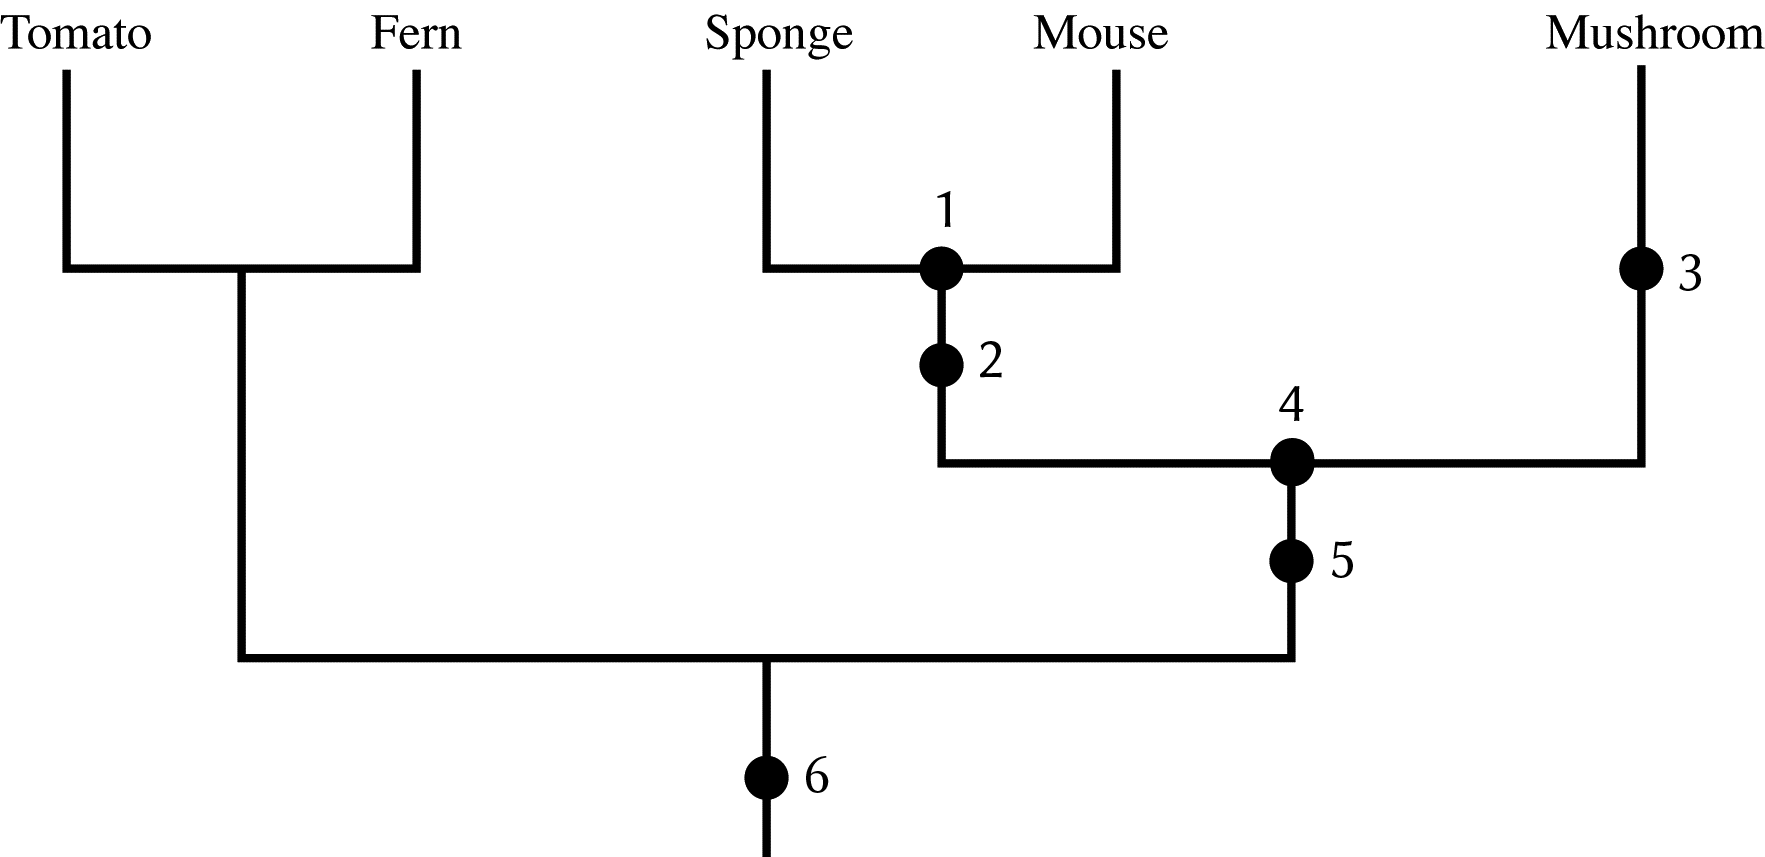
\includegraphics[width=0.45\textwidth]{exam1_tree2}
\end{multicols}
%EndMC

%BeginMC
\question
\begin{multicols}{2}
Small phylogenetic trees are representatives of larger phylogenetic trees. The small trees must convey the same relationships (same ancestors) given by the larger tree. The tree at right shows the relationships among various primates. Which of the following small trees shows a \emph{different} relationship from the primate tree?
\columnbreak
\begin{center}\includegraphics[width=0.3\textwidth]{exam1_big_tree}\end{center}
\end{multicols}

\begin{multicols}{2}
\begin{choices}
\choice \includegraphics[width=0.25\textwidth]{exam1_small_treeA} %EndChoice
\correctchoice \includegraphics[width=0.25\textwidth]{exam1_small_treeD} %EndChoice
\choice \includegraphics[width=0.25\textwidth]{exam1_small_treeC} %EndChoice
\choice \includegraphics[width=0.25\textwidth]{exam1_small_treeB} %EndChoice
\end{choices}
\end{multicols}
%EndMC


%BeginMC
\question
\begin{multicols}{2}
	Phylogenetic trees often represent small subsets of larger phylogenetic trees. Compare the smaller phylogenies (a--d) to the larger phylogeny show below right, then pick which of the smaller phylogenies shows a pattern of relationships that is not consistent with the pattern shown by the larger phylogeny.
	
	\begin{choices}
		\choice 1. %EndChoice
		\choice 2. %EndChoice
		\choice 3. %EndChoice
		\correctchoice 4. %EndChoice
	\end{choices}
	
	\columnbreak
	
	\includegraphics[width=0.4\textwidth]{exam1_tree3a}
\end{multicols}

{\centering\includegraphics[width=0.8\textwidth]{exam1_tree3b}\par}
%EndMC

%%

%BeginMC
\question
Which of these statements about human evolution is correct?  

\begin{choices}
\correctchoice Different species of the genus \textit{Homo} have coexisted at various times throughout hominin evolution.   %EndChoice
\choice The ancestors of \textit{Homo sapiens} were chimpanzees.   %EndChoice
\choice Human evolution has proceeded in an linear fashion from \textit{Australopithecus} to \textit{Homo sapiens.}   %EndChoice
\choice The evolution of upright posture and enlarged brain occurred simultaneously.   %EndChoice
\choice \textit{Australopithecus} was the first group to use projectile hunting tools. %EndChoice
\end{choices}
%EndMC

%BeginMC
\question
The oldest fossil remains of \textit{Homo sapiens} found so far date from about  

\begin{choices}
\choice 8,000–10,000 years ago. %dontshuffle %EndChoice
\choice 50,000–60,000 years ago. %dontshuffle %EndChoice
\correctchoice 200,000–300,000 years ago. %dontshuffle %EndChoice
\choice 1.6–2.0 million years ago. %dontshuffle %EndChoice
\choice 5–6 million years ago. %dontshuffle %EndChoice
\end{choices}
%EndMC

%BeginMC
\question
Why is the discovery of the fossil \textit{Archaeopteryx} significant? It supports the  

\begin{choices}
\correctchoice hypothesis that birds evolved from dinosaurs. %EndChoice
\choice contention that birds are much older than originally thought. %EndChoice
\choice hypothesis that birds evolved feathers before dinosaurs. %EndChoice
\choice hypothesis that most dinosaurs were covered in feathers. %EndChoice
\choice hypothesis that the earliest birds were cold-blooded. %EndChoice  
\end{choices}
%EndMC


%BeginMC
\question
Examination of the fossils of \textit{Archaeopteryx} reveals that, in common with living birds, it had  

\begin{choices}
\choice a long tail containing vertebrae. %EndChoice
\choice feathers.  %EndChoice
\choice teeth.  %EndChoice
\choice both feathers and and a long tail with vertebrae.  %EndChoice
\choice teeth, feathers, and a long tail with vertebrae. %EndChoice
\end{choices}
%EndMC


%BeginMC
\question
Which of these statements about human evolution is correct?  

\begin{choices}
\correctchoice Different species of the genus \textit{Homo} have coexisted at various times throughout hominin evolution.   %EndChoice
\choice The ancestors of \textit{Homo sapiens} were chimpanzees.   %EndChoice
\choice Human evolution has proceeded in an linear fashion from \textit{Australopithecus} to \textit{Homo sapiens.}   %EndChoice
\choice The evolution of upright posture and enlarged brain occurred simultaneously.   %EndChoice
\choice \textit{Australopithecus} was the first group to use projectile hunting tools. %EndChoice
\end{choices}
%EndMC


%BeginMC
\question
Two species that each share an immediate common ancestor are called

\begin{choices}
\correctchoice sister species. %EndChoice
\choice descendant species. %EndChoice
\choice taxa. %EndChoice
\choice branch species. %EndChoice
\choice rooted species. %EndChoice
\end{choices}
%EndMC

%BeginMC
\question
The biological species concept emphasizes

\begin{choices}
\choice the formation of cryptic species.%EndChoice
\choice gene flow between species.%EndChoice
\choice reproductive isolation between populations.%EndChoice
\choice reproductive isolation between species.%EndChoice
\choice the formation of morphologically distinct species.%EndChoice
\end{choices}
%EndMC

%BeginMC
\question
What does the biological species concept use as the primary criterion for determining whether two populations are the same species?

\begin{choices}
\correctchoice gene flow.   %EndChoice
\choice geographic isolation.   %EndChoice
\choice ecological differences.   %EndChoice
\choice morphological similarity.   %EndChoice
\choice allopatric speciation.   %EndChoice
\end{choices}
%EndMC



%BeginMC
\question
Two closely related species of maple trees occur together in the southeastern United States.  Pollen from each species is distributed by the wind.  If the pollen from one species lands on the stigma (female pollen receptor) of the other species but a protein interaction between the pollen and stigma prevents fertilization, then which reproductive barrier keeps the two maple species isolated?

\begin{choices}
\choice mechanical.%EndChoice
\choice behavioral.%EndChoice
\choice habitat.%EndChoice
\correctchoice gametic.%EndChoice
\choice temporal.%EndChoice
\end{choices}
%EndMC

%BeginMC
\question
Two species of \textit{Heliconius} butterflies occupy different habitats but the two species occur together in one area where their habitats are most similar. In this area, the two species often interbreed and hybrid offspring have been observed.  Yet, biologists continue to classify the butterflies as two separate species.  Which of the following observations would provide the best support for classifying the butterflies as two separate species? 

\begin{choices}
\choice The two species are reproductively isolated because they occupy very different habitats.%EndChoice
\choice The two species are cryptic species.%EndChoice
\choice The hybrids are cryptic species.%EndChoice
\correctchoice The hybrids have much lower fitness in the parental habitats.%EndChoice
\choice The two species are morphological species, not biological species.%EndChoice
\choice The two species are biological species, not morphological species.%EndChoice
\end{choices}
%EndMC

%BeginMC
\question
Over time, the movement of people among all countries on Earth has steadily increased. This has altered the course of human evolution by increasing

\begin{choices}
\choice nonrandom mating. %EndChoice
\choice geographic isolation. %EndChoice
\choice genetic drift. %EndChoice
\correctchoice gene flow. %EndChoice
\choice natural selection. %EndChoice
\end{choices}
%EndMC

%BeginMC
\question
Beetle pollinators of a particular plant are attracted to the bright orange flowers. The beetles not only pollinate the flowers, but they mate while inside of the flowers. A mutant version of the plant with red flowers becomes more common over time. A particular variant of the beetle prefers the red flowers to the orange flowers. Over time, these two beetle variants diverge from each other to such an extent that interbreeding is no longer possible. What kind of speciation has occurred in this example, and what has driven it?

\begin{choices}
\choice allopatric speciation; ecological isolation%EndChoice
\correctchoice sympatric speciation; ecological isolation%EndChoice
\choice allopatric speciation; temporal isolation%EndChoice
\choice sympatric speciation; temporal isolation%EndChoice
\choice allopatric speciation; behavioral isolation%EndChoice
\choice sympatric speciation; gametic isolation%EndChoice
\end{choices}
%EndMC

%BeginMC
\question
Male frogs give calls that attract female frogs to approach and mate. Researchers examined mating calls of closely related tree frogs in South America. If reinforcement is occurring, what would you expect if you compare the calls of the two species in zones of sympatry versus zones of allopatry? 

\begin{choices}
\correctchoice Calls would be more different in areas of sympatry. %EndChoice
\choice Calls would be about the same in both areas. %EndChoice
\choice Calls would be more similar in areas of sympatry. %EndChoice
\choice Calls were become more similar due to fusion. %EndChoice
\end{choices}
%EndMC

%BeginMC
\question
A hybrid zone is properly defined as 

\begin{choices}
\correctchoice an area where mating occurs between members of two closely related species, producing at least some viable offspring. %EndChoice
\choice an area where the ranges of two closely related species overlap, but do not interbreed. %EndChoice
\choice a zone where the two closely related species remain distinct through hybrid fusion. %EndChoice
\choice an area where members of two closely related species intermingle, but gene flow is prevented by prezygotic barriers. %EndChoice
\choice an area where members of two closely related species intermingle, but gene flow is prevented by allopatric barriers. %EndChoice
\end{choices}
%EndMC


%BeginMC
\question
Lakes in east Africa have been suffering pollution, causing a decline in species diversity of cichlid fishes. This decline in diversity is most likely due to

\begin{choices}
\choice reinforcement. %EndChoice
\correctchoice fusion. %EndChoice
\choice stability. %EndChoice
\choice hybrid inviability. %EndChoice
\choice hybrid sterility. %EndChoice
\end{choices}
%EndMC

%BeginMC THINK CAREFULLY ABOUT USING THIS ONE.
\question
Suppose that a group of male pied flycatchers migrated from a region where there were no collared flycatchers to a region where both species were present. Assuming events like this are very rare, which of the following scenarios is \emph{least} likely?

\begin{choices}
\choice Migrant pied males would produce fewer offspring than would resident pied males. %EndChoice
\choice Pied females would rarely mate with collared males. %EndChoice
\choice Migrant males would mate with collared females more often than with pied females. %EndChoice
\choice The frequency of hybrid offspring would decrease. %EndChoice
\end{choices}
%EndMC


%BeginMC
\question
A hypothetical island lies far from any other landmasses. There are many different types of plants, but only one animal, a beetle, that can fly or walk from plant to plant and feeds by chewing leaves. Given that the beetle is not exploiting all of the resources on the island, which morphological change would be most likely to trigger an adaptive radiation of the beetles?

\begin{choices}
\choice a change in wing shape that improves flight speed. %EndChoice
\choice an additional segment on a pair of legs. %EndChoice
\correctchoice a mouthpart that can pierce fruits and seeds. %EndChoice
\end{choices}
%EndMC


%BeginMC
\question
The regulatory gene that determines where eyes will appear is

\begin{choices}
\correctchoice \textit{Pax6} %EndChoice
\choice \textit{Antp} %EndChoice
\choice \textit{Shh} %EndChoice
\choice \textit{Ubx} %EndChoice
\choice \textit{Hox} %EndChoice
\end{choices}
%EndMC

%BeginMC
\question
The regulatory gene that determines whether a fly will have legs or antennae on the head is

\begin{choices}
\correctchoice \textit{Antp} %EndChoice
\choice \textit{Pax6} %EndChoice
\choice \textit{Shh} %EndChoice
\choice \textit{Ubx} %EndChoice
\choice \textit{Hox} %EndChoice
\end{choices}
%EndMC


%BeginMC
\question
A change in the body location where two \textit{Hox} genes are expressed caused swimming appendages to evolve into feeding appendages in crabs and other crustaceans. This type of genetic change is an example of

\begin{choices}
\correctchoice a change in a toolkit gene that altered the arrangement of parts in the body plan. %EndChoice
\choice heterochrony that caused a difference in developmental timing. %EndChoice
\choice allometry that caused the swimming appendages to grow more slowly so they could be used for feeding. %EndChoice
\choice paedomorphosis that caused the adult to retain the juvenile feeding appendage. %EndChoice
\choice an adaptation to living in an quiet aquatic environment where fewer swimming appendages are needed. %EndChoice
\end{choices}
%EndMC



%BeginMC
\question
A genetic change that caused a certain \textit{Hox} gene to be expressed along the tip of a vertebrate limb bud instead of farther back helped make possible the  evolution of the tetrapod limb. This type of change is an example of 
\begin{choices}
\choice the influence of environment on development.%EndChoice
\choice paedomorphosis.%EndChoice
\correctchoice a change in a developmental gene that altered the organization of body parts.%EndChoice
\choice heterochrony.%EndChoice
\choice allometry.%EndChoice
\end{choices}
%EndMC

%BeginMC
\question
The most important feature that permits a gene to act as a molecular clock is 

\begin{choices}
\correctchoice a reliable average rate of mutation. %EndChoice
\choice a large number of base pairs. %EndChoice
\choice being acted upon by natural selection. %EndChoice
\choice a recent origin by a gene-duplication event. %EndChoice
\choice that it is a conserved gene. %EndChoice
\end{choices}
%EndMC

	%% FIX ANSWER CHOICES.
%BeginMC
\question
Chimpanzees and humans may be as much as 98.5\% genetically identical.  A likely reason for the large phenotypic difference between chimps and humans is

\begin{choices}
\correctchoice a difference in the developmental expression and timing of toolkit genes. %EndChoice
\choice the similar genotype interacting with the different physical environments occupied by each species. %EndChoice
\choice a large difference in the types of genes found in each species. %EndChoice
\choice paedomorphic development of most human traits. %EndChoice
\choice allometric development of most human traits. %EndChoice
\choice heterochronic development of most chimpanzee traits. %EndChoice
\end{choices}
%EndMC

